%%%%%%%%%%%%%%%%%%%%%%%%%%%%%%%%%%%%%%%%%%%%%%%%%%%%%%%%%%%%%%%%%%%%%%%%%%%%%%%%%%
\begin{frame}[fragile]\frametitle{}
\begin{center}
{\Large Applications}
\end{center}
\end{frame}




%%%%%%%%%%%%%%%%%%%%%%%%%%%%%%%%%%%%%%%%%%%%%%%%%%%%%%%%%%%%%%%%%%%%%%%%%%%%%%%%%%
\begin{frame}[fragile]\frametitle{Sentiment Analysis}

Sentiment analysis involves analyzing a text to determine the sentiment, whether it is positive, negative, or neutral. 

{\tiny (Ref: LangChain: New NLP/NLU Shining Armor - Sandeep Singh)}

\begin{lstlisting}
from langchain import LangChain

# Initialize LangChain object
lc = LangChain()

# Define input text
input_text = "I love LangChain! It's the best NLP library I've ever used."

# Perform sentiment analysis
sentiment = lc.sentiment(input_text)

# Print the sentiment
print(sentiment)
\end{lstlisting}	  

\end{frame}


%%%%%%%%%%%%%%%%%%%%%%%%%%%%%%%%%%%%%%%%%%%%%%%%%%%%%%%%%%%%%%%%%%%%%%%%%%%%%%%%%%
\begin{frame}[fragile]\frametitle{Named Entity Recognition (NER)}

Named Entity Recognition is the process of identifying and categorizing named entities such as people, places, organizations, and dates in text data.

{\tiny (Ref: LangChain: New NLP/NLU Shining Armor - Sandeep Singh)}

\begin{lstlisting}
from langchain import LangChain

# Initialize LangChain object
lc = LangChain()

# Define input text
input_text = "Microsoft is acquiring Nuance Communications for $19.7 billion."

# Perform NER
entities = lc.ner(input_text)

# Print the entities
print(entities)
\end{lstlisting}	  

\end{frame}

%%%%%%%%%%%%%%%%%%%%%%%%%%%%%%%%%%%%%%%%%%%%%%%%%%%%%%%%%%%%%%%%%%%%%%%%%%%%%%%%%%
\begin{frame}[fragile]\frametitle{Text Summarization}

Text summarization is the process of reducing a text document to a shorter version while retaining its most important information.

{\tiny (Ref: LangChain: New NLP/NLU Shining Armor - Sandeep Singh)}

\begin{lstlisting}
from langchain import LangChain

# Initialize LangChain object
lc = LangChain()
input_text = "In recent years, natural language processing (NLP) has seen quick progress and significant breakthroughs in various domains, including machine translation, sentiment analysis, and text summarization. Text summarization is the process of reducing a text document to a shorter version while retaining its most important information. There are two types of text summarization: extractive and abstractive. Extractive summarization involves selecting important sentences or phrases from the original document, while abstractive summarization involves generating new sentences to summarize the content."
max_length = 50

summary = lc.summarize(input_text, max_length)
print(summary)
\end{lstlisting}	  

\end{frame}

%%%%%%%%%%%%%%%%%%%%%%%%%%%%%%%%%%%%%%%%%%%%%%%%%%%%%%%%%%%%%%%%%%%%%%%%%%%%%%%%%%
\begin{frame}[fragile]\frametitle{Part-of-Speech (POS) Tagging}

Part-of-Speech (POS) Tagging is the process of identifying and tagging the part of speech of each word in a sentence. 

{\tiny (Ref: LangChain: New NLP/NLU Shining Armor - Sandeep Singh)}

\begin{lstlisting}
from langchain import LangChain

# Initialize LangChain object
lc = LangChain()

# Define input text
input_text = "I am learning natural language processing using LangChain."

# Perform POS tagging
pos_tags = lc.pos_tag(input_text)

# Print the POS tags
print(pos_tags))
\end{lstlisting}	  

\end{frame}

%%%%%%%%%%%%%%%%%%%%%%%%%%%%%%%%%%%%%%%%%%%%%%%%%%%%%%%%%%%%%%%%%%%%%%%%%%%%%%%%%%
\begin{frame}[fragile]\frametitle{Text Similarity}

Text similarity is the process of measuring how similar two pieces of text are to each other.

{\tiny (Ref: LangChain: New NLP/NLU Shining Armor - Sandeep Singh)}

\begin{lstlisting}
from langchain import LangChain

# Initialize LangChain object
lc = LangChain()

# Define two input texts
input_text1 = "I love playing basketball."
input_text2 = "Basketball is my favorite sport."

# Compute text similarity
similarity = lc.text_similarity(input_text1, input_text2)

# Print the similarity score
print(similarity)
\end{lstlisting}	  

\end{frame}

%%%%%%%%%%%%%%%%%%%%%%%%%%%%%%%%%%%%%%%%%%%%%%%%%%%%%%%%%%%%%%%%%%%%%%%%%%%%%%%%%%
\begin{frame}[fragile]\frametitle{Language Detection}

Language detection is the process of identifying the language of a given text.

{\tiny (Ref: LangChain: New NLP/NLU Shining Armor - Sandeep Singh)}

\begin{lstlisting}
from langchain import LangChain

# Initialize LangChain object
lc = LangChain()

# Define input text
input_text = "Bonjour, comment ca va?"

# Perform language detection
language = lc.detect_language(input_text)

# Print the detected language
print(language)
\end{lstlisting}	  

\end{frame}

%%%%%%%%%%%%%%%%%%%%%%%%%%%%%%%%%%%%%%%%%%%%%%%%%%%%%%%%%%%%%%%%%%%%%%%%%%%%%%%%%%
\begin{frame}[fragile]\frametitle{Text Generation}

Text generation is the process of generating new text based on a given input or context. 

{\tiny (Ref: LangChain: New NLP/NLU Shining Armor - Sandeep Singh)}

\begin{lstlisting}
from langchain import LangChain

# Initialize LangChain object
lc = LangChain()

# Define input context
input_context = "The quick brown fox jumps over the"

# Generate new text
generated_text = lc.generate_text(input_context, length=50)

# Print the generated text
print(generated_text)
\end{lstlisting}	  

\end{frame}


%%%%%%%%%%%%%%%%%%%%%%%%%%%%%%%%%%%%%%%%%%%%%%%%%%%%%%%%%%%%%%%%%%%%%%%%%%%%%%%%%%
\begin{frame}[fragile]\frametitle{Exercise}

 Building a Q\&A system
 
  \begin{itemize}
    \item \textbf{Objective}: Create a Q\&A system for official holidays in the UAE.
    \item \textbf{Components Overview}:
      \begin{enumerate}
        \item \textbf{Prompt}: Define queries related to UAE holidays.
        \item \textbf{Agents}: Utilize agents for tasks like language understanding and information retrieval.
        \item \textbf{Tools}: Leverage tools for data manipulation and processing.
        \item \textbf{Memory}: Implement memory for context retention and follow-up interactions.
      \end{enumerate}
    \item \textbf{Schema Development}:
      \begin{itemize}
        \item Visual representation of components interconnection.
      \end{itemize}
    \item \textbf{Schema Components}:
      \begin{enumerate}
        \item \textbf{Prompt Handling}: Formulate questions about UAE holidays.
        \item \textbf{Agent Integration}: Connect language understanding agents.
        \item \textbf{Tool Application}: Employ tools for data manipulation.
        \item \textbf{Memory Usage}: Implement memory for context retention.
      \end{enumerate}
  \end{itemize}

Build your own solution, prep a short demo reel, post on LinkedIn and tag me!!

{\tiny Ready solution: https://colab.research.google.com/drive/1svn1BPfIiUL-82P4Rv\_smoTPPyoeuWfa\#scrollTo=gXypMluAjBME}
\end{frame}

%%%%%%%%%%%%%%%%%%%%%%%%%%%%%%%%%%%%%%%%%%%%%%%%%%%%%%%%%%%%%%%%%%%%%%%%%%%%%%%%%%
\begin{frame}[fragile]\frametitle{Architecture}

  
			\begin{center}
			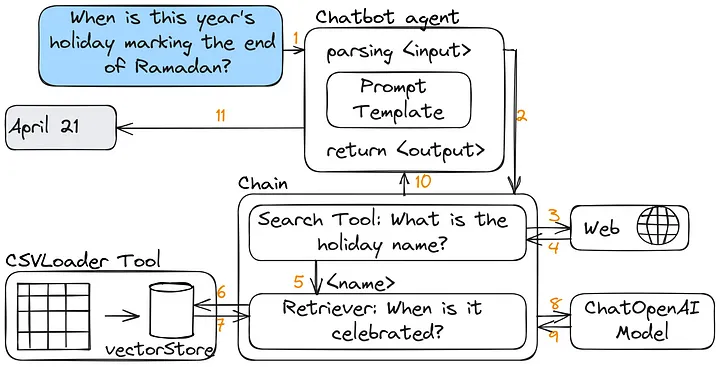
\includegraphics[width=\linewidth,keepaspectratio]{langchain14}
			\end{center}	  


			{\tiny (Ref: LangChain 101: Part 1. Building Simple Q\&A App - Ivan Reznikov)}


\end{frame}


%%%%%%%%%%%%%%%%%%%%%%%%%%%%%%%%%%%%%%%%%%%%%%%%%%%%%%%%%%%%%%%%%%%%%%%%%%%%%%%%%%
\begin{frame}[fragile]\frametitle{Data}

  The data we’ll be using can be found at the following website, as shown in the table below:
  
  https://publicholidays.ae/2023-dates/
  
\begin{lstlisting}
+--------+-----+-----------------------------+
|  Date  | Day |           Holiday           |
+--------+-----+-----------------------------+
| 1 Jan  | Sun | New Year's Day              |
| 20 Apr | Thu | Eid al-Fitr Holiday         |
| 21 Apr | Fri | Eid al-Fitr                 |
| 22 Apr | Sat | Eid al-Fitr Holiday         |
| 23 Apr | Sun | Eid al-Fitr Holiday         |
| 27 Jun | Tue | Arafat Day                  |
| 28 Jun | Wed | Eid al-Adha                 |
| 29 Jun | Thu | Eid al-Adha Holiday         |
| 30 Jun | Fri | Eid al-Adha Holiday         |
| 21 Jul | Fri | Islamic New Year            |
| 29 Sep | Fri | Prophet Muhammad's Birthday |
| 1 Dec  | Fri | Commemoration Day           |
| 2 Dec  | Sat | National Day                |
| 3 Dec  | Sun | National Day Holiday        |
+--------+-----+-----------------------------+
\end{lstlisting}	  


\end{frame}

%%%%%%%%%%%%%%%%%%%%%%%%%%%%%%%%%%%%%%%%%%%%%%%%%%%%%%%%%%%%%%%%%%%%%%%%%%%%%%%%%%
\begin{frame}[fragile]\frametitle{Testing}


  
\begin{lstlisting}
query = "Are there any holidays in March?"
print_response_for_query(query)

> Finished chain.
Based on the data provided, there are no holidays in March.

query = "Sorry, I meant December"
print_response_for_query(query)

> Finished chain.
Based on the data provided, there are two official holidays in December 
for the UAE. The first one is Commemoration Day on December 1st, which 
falls on a Friday. The second one is National Day on December 2nd, which 
falls on a Saturday. Additionally, there is a National Day Holiday on 
December 3rd, which falls on a Sunday.
\end{lstlisting}	  


\end{frame}



